\chapter{Study Management}

\section{Study Aggregate}

 The Study aggregate is used to configure a study. It defines the valid types
 of specimens that can be collected, when they are to be collected from
 participants, and how collected specimens are processed.

\begin{figure}[h]
  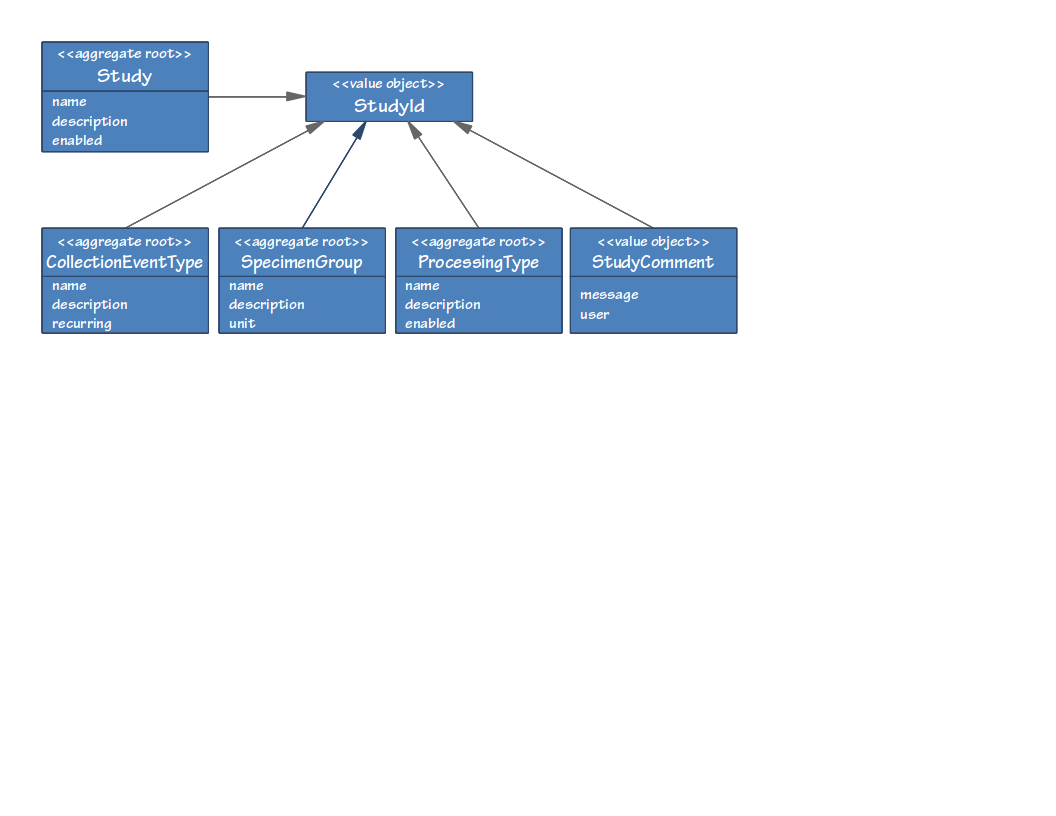
\includegraphics[trim={9mm 104mm 80mm 9mm}, clip,
    width=1\textwidth]{images/study-aggregate}
  \caption{Study aggregate}
  \label{fig:study-aggregate}
\end{figure}

\begin{description}[listparindent=\parindent]

  \item[\entitytarget{Study}] \hfill \\ Represents a collection of participants and
    specimens collected for a particular research study.

    A study can be enabled or disabled. When disabled, changes to its
    configuration are possible but patients and specimens cannot be added. When
    enabled, no further configuration changes are allowed, and participants and
    specimens can be added.

    A study may have one or more comments assigned to it during it's lifetime.

  \item[\entitytarget{SpecimenGroup}] \hfill \\ Ownership, summary, storage,
    and classification information that applies to an entire group or
    collection of \entitylink{Specimen}s.

    The anatomical source, preservation medium and specimen type are defined
    using other value objects discussed in Section \ref{sec:specimen-group}.

    This entity is used to record the specimen types used by the study. It can
    specify the specimens collected from participants, and the asscociations to
    the specimens that are processed from them.

  \item[\entitytarget{CollectionEventType}] \hfill \\ A classification name,
    unique to the \entitylink{Study}, for a visit by the study's
    participants. One or more of these can be defined per study. Each
    collection event type has a number specimen groups (see
    \valobjlink{SpecimenGroupCollectionEventType}).

  \item[\entitytarget{ProcessingType}] \hfill \\ Describes a regularly
    performed procedure with a unique name (within its
    \entitylink{Study}). There should be one or more associated
    \entitylink{SpecimenProcesingLinkType}s that (1) further define legal
    procedures and (2) allow logging of procedures performed on different types
    of \entitylink{Specimen}s.

  \item[\entitytarget{}] \hfill \\

  \item[\entitytarget{}] \hfill \\


\end{description}

\subsection{SpecimenGroup}
\label{sec:specimen-group}

The SpecimenGroup entity is composed of other value objects as shown in Figure
\ref{fig:specimen-group}.

\begin{figure}[h]
  \centering
  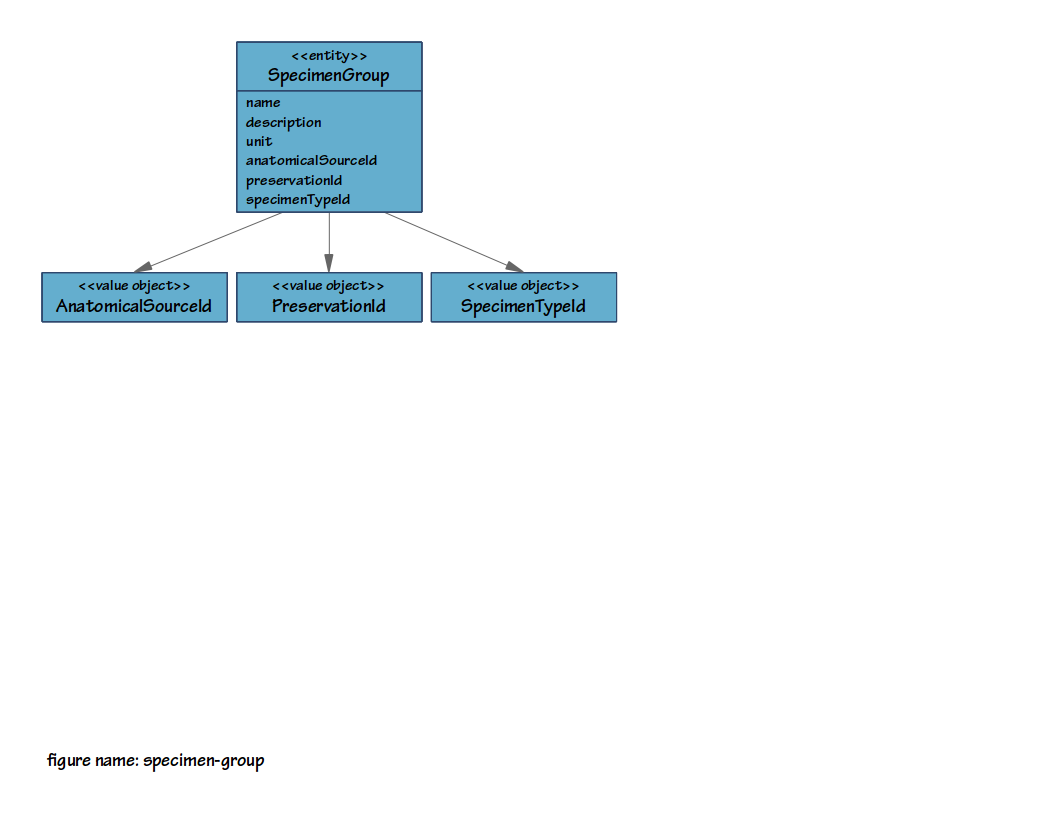
\includegraphics[trim={9mm 110mm 80mm 9mm}, clip,
    width=0.9\textwidth]{images/specimen-group}
  \caption{SpecimenGroup entity}
  \label{fig:specimen-group}
\end{figure}

\begin{description}

  \item[\valobjtarget{Preservation}] \hfill \\ Describes how a
    \entitylink{Specimen} should be preserved/stored by describing temperature
    requirements, as well as a preservation method (see
    \valobjlink{PreservationType}).

  \item[\valobjtarget{PreservationType}] \hfill \\ A standardised set of
    methods for preserving and storing \entitylink{Specimen}s.  Potential
    examples include: frozen specimen, RNA later, fresh specimen, slide, etc.

  \item[\valobjtarget{SpecimenType}] \hfill \\ A standardised set of
    classifications that describe \emph{what} a \entitylink{Specimen}
    is. Potential examples include: urine, whole blood, plasma, nail, protein,
    etc.

\end{description}

\subsection{CollectionEventType}
\label{sec:collection-event-type}

The \texttt{\textbf{\valobjtarget{SpecimenGroupCollectionEventType}}} value
object is used to define which types of specimens (i.e. which
\valobjlink{SpecimenGroup}s) need to be collected as part of a
\entitylink{CollectionEventType}. See Figure \ref{fig:collection-event-type}.

\begin{figure}[h]
  \centering
  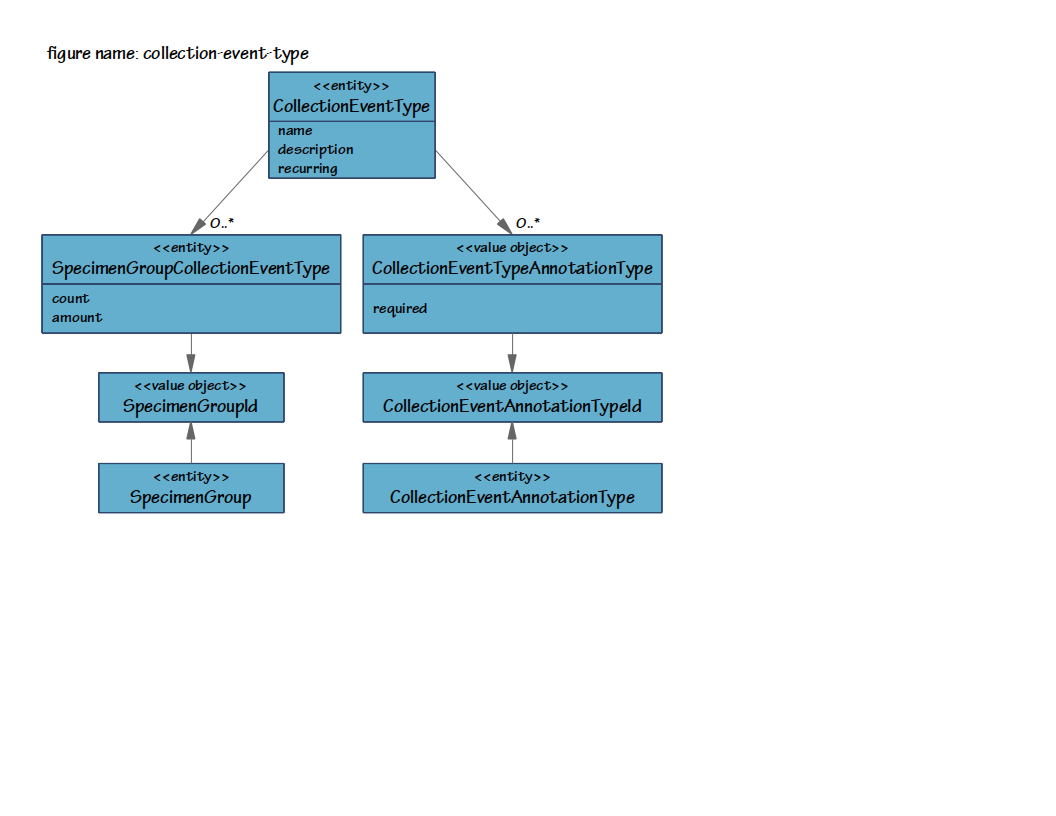
\includegraphics[trim={9mm 118mm 158mm 9mm}, clip,
    width=0.6\textwidth]{images/collection-event-type}
  \caption{Associating collection event types and specimen groups}
  \label{fig:collection-event-type}
\end{figure}

\subsection{ProcessingType}
\label{sec:Processing-type}

The \texttt{\textbf{\valobjtarget{SpecimenLinkType}}} represents a regularly
performed processing procedure involving two \entitylink{Specimen}s: an input,
which must be in a specific \valobjlink{SpecimenGroup}, and an output, which
must be in a specific \valobjlink{SpecimenGroup}.

\begin{figure}[h]
  \centering
  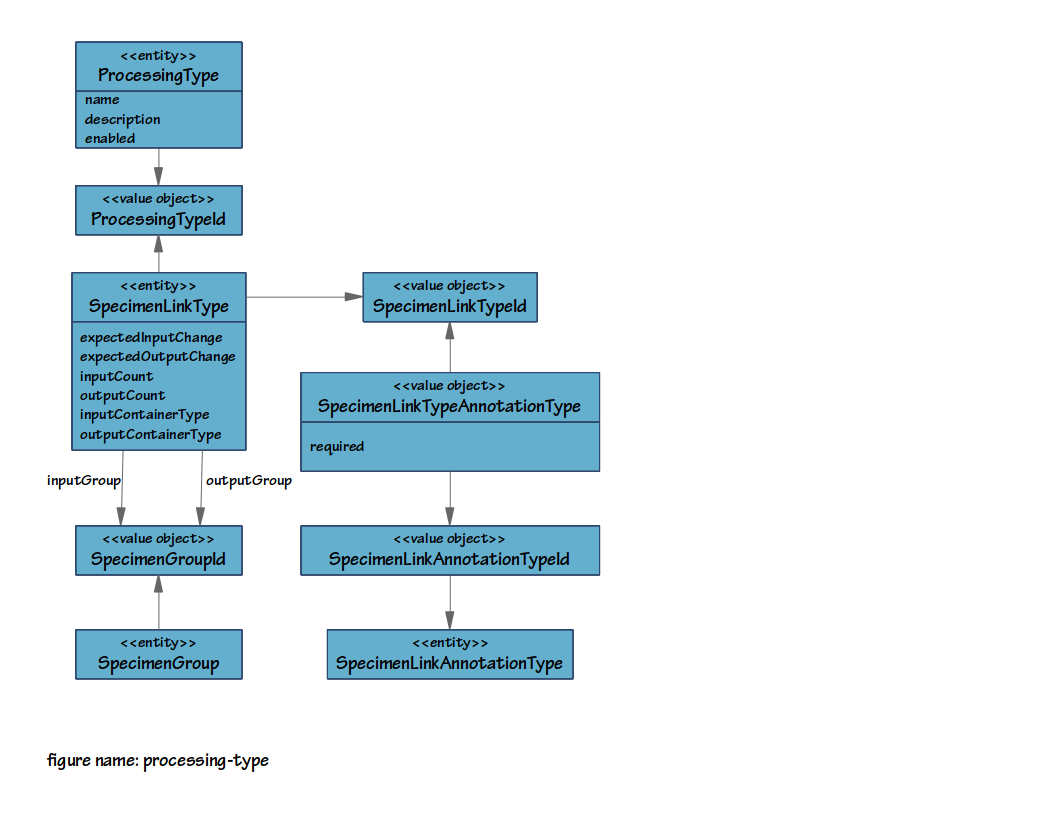
\includegraphics[trim={9mm 120mm 172mm 9mm}, clip,
    width=0.6\textwidth]{images/processing-type}
  \caption{Association processing types with specimen groups}
  \label{fig:processing-type}
\end{figure}

